\documentclass[]{article}
\usepackage[utf8]{inputenc}
\usepackage{natbib}
\usepackage{graphicx}
\usepackage{geometry}
\usepackage{hyperref}






\geometry{
	a4paper,
	total={170mm,257mm},
	left=20mm,
	top=20mm,
}

%opening
\title{Progetto di Algoritmi Avanzati  	
		\\ \large Capacitated Vehicle Routing Problem 
		 \\  Algoritmi: Costruttivi, a 2 Fasi e Genetici}
	 

\author{Giulio Pilotto - Matricola:1140718}

\date{Luglio 2019}

	

\begin{document}
	



\maketitle


\begin{abstract}

Questo elaborato presenta il progetto di Algoritmi Avanzati sottomesso al prof. Bresolin dell'Università di Padova.
Il progetto richiede di implementare almeno 2 algoritmi che risolvono istanze di : Capacitated Vehicle Routing Problem.
Nel seguente elaborato oltre ad implementare i 2 algoritmi richiesti , il primo come metodo costruttivo; Clarke and Wright e il secondo come metodo a 2 fasi:ClusterFirst - Route Second per il quale sono state implementate due tecniche di routing: Nearest-Neighbourn e Dijkastra.
Sono stati implementati altri 2 algoritmi uno che cade sempre nella classe dei metodi a 2 fasi: RouteFirst - ClusterSecond, e un altro che cade nella categoria degli algoritmi metauristici detti anche algoritmi genetici.
Inoltre, è stato implementato un metodo di selezione dei centroidi che tiene conto sia della distanza dal deposito sia della distanza inter-cluster.
Tutti gli algoritmi sono stati testati sulle 16 istanze fornite dalla libreria TSPLIB95.
I risultati confermano che a fronte di una minore accuratezza di una soluzione rispetto all'ottimo ma una maggiore richiesta di risorse in termini di tempo, possono portare a soluzioni ben approssimate.
In particolare scegliere i centrodi con il metodo RadiusRadar permette di guadagnare qualche decimo a fronte di un tempo inore.
Le soluzioni posso essere migliorate attrverso gli algoritmi genetici che fungono da esploratori di uno spazion locale.

\end{abstract}

\section{Introduzione}
Con la nascita dei nuovi servizi per il cliente, che danno assistenza e portao i prodotti direttamente sulla soglia di casa (es:Amazon Prime), la gestione della logistica predilige gran parte degli investimenti.
Questo fatto diventa ancor più importante se diamo un occhiata ai dati forniti dall' Associazione Nazionale Filiera Industria Automobilistica (ANFIA) nel 2017 \ref{fig:ITA28} , dove viene sottolineato che i camion movimentano l'80$\%$ delle merci su terra \cite{ANFIA2017}. 
Gli investimenti non riguardano solo le strutture o gli strumenti fisici, ma soprattutto i software per la gestione e l'ottimizzazione  della distribuzione dei beni.
Grazie all'informatizzazione dei processi da parte del nuovo programma di industrializzazione chiamato "industria 4.0", si può godere di banche dati ricche ed aggiornate, attraverso le quali, possono essere implementate tecniche di ricerca operativa e ottimizzazione.

Il Vehicle Routing Problem \textbf{(VRP)}  è un classe reale di problemi di soddisfacimento di vincoli, in inglese detto anche Constraint Satisfaction Problem \textbf{(COP)}.
Alla fine degli anni cinquanta Dantzig and Ramser hanno formalizzato il problema \cite{dispatching} che riguarda la distribuzione di benzina da un deposito princiapale ad un grande numero di stazioni di servizio.
Da quel momento l'interesse nei problemi VRP è evoluto da un piccolo gruppo di matematici ad un grande gruppo di ricercatori da differenti discipline ancora oggi coinvolti.


VRP consiste nell'ottimizzare l'uso di un insieme di veicoli per prelevare della merce da uno o più depositi e consegnarle presso stazioni che richiedono una certa quantità di merce.
Le stazioni , i depositi sono distribuiti in uno spazio rappresentato da delle distanze. I mezzi si spostano percorrendo tali distanze, che possono essere rappresentate in maniera diversa.
La maggioranza the problemi reali sono sepsso più complessi del classico VRP. Quindi in pratica VRP è aumentato con dei vincoli, come ad esempio la capacità del veicolo: dove ogni veicolo è caratterizzato da una capacità limitata di carico delle merci, passando quindi da VRP a \textbf{Capacitated - VRP}.
Gli obiettivi sono molteplici:
\begin{itemize}
	\item Minimizzare dei costi di trasporto (istanze percorse, consumo di carburante)
	\item Minimizzare il numero di veicoli
	\item Rispettare il vincolo di capacità imposto  sui veicoli.
	\item Un percorso deve essere assegnato ad un solo veicolo.
\end{itemize}


\begin{figure}[h!]
	\centering
	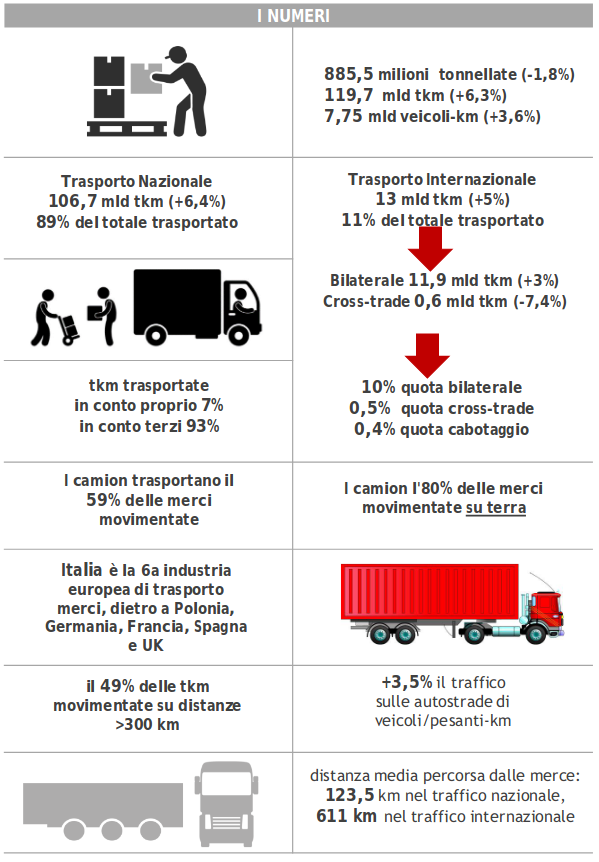
\includegraphics[scale=0.50]{images/ITA28.png}
	\caption{ Italia, traffico merci su strada, ANFIA su dati ISTAT 2017 }
	\label{fig:ITA28}
\end{figure}

VRP è un problema di ottimizzazione combinatoria NP hard,che può essere risolto esattamente trovando l'ottimo solo per piccole istanze del problema. In ogni caso gli approcci euristici che non garantiscono l'ottimalità, forniscono ottimi risultati in pratica.
Negli ultimi 30 anni sono stati applicati anche dei metodimeta-euristici che hanno mostrato una nuova direzioe alla ricerca sulla famiglia di problemi VRP  



\bibliographystyle{unsrt}
\bibliography{biblio}

\section{Related Works}

\end{document}









